%%%%%%%%%%%%%%%%%%%%%%%%%%%%%%%%%%%%%%%%%%%%%%%%%%%%%%%%%%%%%%%%%%%%%%%%%%%%%%%
% Mid Project Demonstration
% Application of Machine Learning Techniques to Next Generation Quality Control
% Aberystwyth University
% Sam Nicholls <msn@aber.ac.uk>
%%%%%%%%%%%%%%%%%%%%%%%%%%%%%%%%%%%%%%%%%%%%%%%%%%%%%%%%%%%%%%%%%%%%%%%%%%%%%%%

\documentclass{beamer}

\mode<presentation>
{
  \setbeamercovered{transparent}
  \usepackage{lmodern}
  \usetheme{CambridgeUS}
  %\usecolortheme[RGB={40,75,255}]{structure}
  \usecolortheme{dolphin}
  \useoutertheme[compress,subsection=false]{miniframes}
  \setbeamertemplate{items}[ball]
  \setbeamertemplate{blocks}[rounded]
  \setbeamersize{text margin left=5mm, text margin right=5mm}
}

\mode<handout>{\beamertemplatesolidbackgroundcolor{black!5}}
\usepackage{amsfonts}
\usepackage{amsthm,amsmath}
\usepackage{graphicx}

\usepackage[english]{babel}
\usepackage[latin1]{inputenc}
\usepackage{times}
\usepackage[T1]{fontenc}
% Note that the encoding and the font should match.
% If T1 does not look nice, try deleting the line with the fontenc.

\setbeamertemplate{navigation symbols}{}


%%%%%%%%%%%%%%%%%%%%%%%%%%%%%%%%%%%%%%%%%%%%%%%%%%%%%%%%%%%%%%%%%%%%%%%%% Title
\title{Mid Project Demonstration}
\subtitle{Application of Machine Learning Techniques\\
    to Next Generation Sequencing Quality Control}

\author[Sam Nicholls]{Sam Nicholls\\\tiny{msn}}
\institute[Aberystwyth University]{
    Department of Computer Science\\
    Aberystwyth University
}
\date{\today}

\begin{document}
\begin{frame}
    \titlepage
\end{frame}


%%%%%%%%%%%%%%%%%%%%%%%%%%%%%%%%%%%%%%%%%%%%%%%%%%%%%%%%%%%%%%%%%%%%%%%%% Intro
\section{Introduction}
\subsection{Introduction}

\begin{frame}[t]
\frametitle{Next Generation Sequencing}
    \uncover<1>{
        \begin{beamerboxesrounded}[shadow=true]{}
            \begin{center}
                What is Next Generation Sequencing?
            \end{center}
        \end{beamerboxesrounded}
        \begin{itemize}
            \item Major and rapid advances in genetic sequencing hardware
            \item Massively parallel; billions of simultaneous chemical reactions
            \item Both time and cost of genetic analysis has reduced
        \end{itemize}
    }

    \uncover<2>{
        \vskip 0.5cm
        \begin{beamerboxesrounded}[shadow=true]{}
            \begin{center}
                Why this project?
            \end{center}
        \end{beamerboxesrounded}
        \begin{itemize}
            \item Processes are complex and open to error
            \item Quality control is an essential step
            \item Must be able to assure confidence for downstream results
        \end{itemize}
    }
\end{frame}


%%%%%%%%%%%%%%%%%%%%%%%%%%%%%%%%%%%%%%%%%%%%%%%%%%%%%%%%%%%%%%%%%%%%%%%%%% Aims
\section{Aims}
\subsection{Aims}

\begin{frame}[t]
\frametitle{Aims}
    \begin{beamerboxesrounded}[shadow=true]{}
        \begin{center}
            Report on state of the current quality control system at Sanger
        \end{center}
    \end{beamerboxesrounded}
    \uncover<1>{
        \begin{itemize}
            \item Working with Sanger Institute's Human Gentics Informatics Team
            \item \texttt{auto\_qc} classifies samples as pass, fail or warn
            \item Current classifier consists of hard-coded simple thresholds
            \item \texttt{auto\_qc} also requires timely human intervention
        \end{itemize}
    }
    \uncover<2>{
        \vskip 0.5cm
        \begin{beamerboxesrounded}[shadow=true]{}
            \begin{center}
                Goals
            \end{center}
        \end{beamerboxesrounded}
        \begin{itemize}
            \item Apply learning techniques to replicate current human rules
            \item Attempt to improve efficiency of current "warning" handling
            \item Identify new or unused parameters that improve classification
        \end{itemize}
    }
\end{frame}


\begin{frame}[t]
\frametitle{Aims}
    \begin{beamerboxesrounded}[shadow=true]{}
        \begin{center}
            Identify lanelet properties that affect downstream variant calling
        \end{center}
    \end{beamerboxesrounded}
    \uncover<1>{
        \begin{itemize}
            \item For better QC we need an idea of "good" and "bad"
            \item How does quality affect analyses performed after sequencing?
        \end{itemize}
    }
    \uncover<2>{
        \vskip 0.5cm
        \begin{beamerboxesrounded}[shadow=true]{}
            \begin{center}
                Goals
            \end{center}
        \end{beamerboxesrounded}
        \begin{itemize}
            \item Will leaving out a sample during variant calling affect the result?
            \item Select a "representative" region of the human genome for analysis
            \item Compare calls on whole genome results to GWAS "SNP chips"
            \item Determine what is actually "good" and "bad" for QC
        \end{itemize}
    }
\end{frame}


%%%%%%%%%%%%%%%%%%%%%%%%%%%%%%%%%%%%%%%%%%%%%%%%%%%%%%%%%%%% QC Report Progress
\section{QC Report Progress}
\subsection{QC Report Progress}

\begin{frame}[t]
\frametitle{Analysis of Current QC System}
    \begin{beamerboxesrounded}[shadow=true]{}
        \begin{center}
            Samples, Lanes and Lanelets (Oh my!)
        \end{center}
    \end{beamerboxesrounded}

    \begin{columns}[c]
    \column{3.0cm}
        \begin{beamerboxesrounded}[shadow=true]{}
            \begin{center}
                \resizebox{1.0\textwidth}{!}{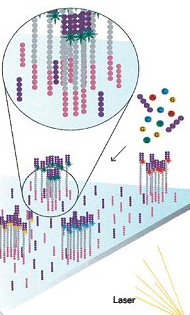
\includegraphics{img/flowcell7.png}}
                {\tiny{Illumina DNA Synthesis}}
            \end{center}
        \end{beamerboxesrounded}
    \column{9.0cm}
        \begin{itemize}
            \item Illumina HiSeq hardware; eight \textbf{lane} flowcell
            \item A \textbf{sample} is a distinct DNA specimen
            \item Samples are prepared with barcodes and amplified across multiple lanes
            \item The amplification process creates millions of clusters in each lane
            \item A lane thus contains more than one sample and samples can be 
                spread across multiple lanes
            \item A \textbf{lanelet} represents the aggregate of all clusters 
                in one particular lane that match the barcode of a particular sample
        \end{itemize}
    \end{columns}
    \vskip 0.2cm
    {\tiny{\textbf{Image} Harvard University Informatics and Scientific Applications: 
        Illumina Sequencing Technology. http://bit.ly/1lMb4KG}}
\end{frame}

\begin{frame}[t]
\frametitle{Analysis of Current QC System}
    \begin{beamerboxesrounded}[shadow=true]{}
        \begin{center}
            Data Access
        \end{center}
    \end{beamerboxesrounded}
    \begin{itemize}
        \item Access to two of the largest studies at the institute
        \item 13,455 "lanelets"; aggregated clusters of a sample in one lane
        \item \texttt{auto\_qc} \textbf{pass} 9,154 (68\%), 
            \textbf{fail} 1,542 (11\%) \textbf{warn} 2,759 (21\%)
        \item Possible access to another large data set on the horizon
    \end{itemize}

    \vskip 0.5cm

    \begin{beamerboxesrounded}[shadow=true]{}
        \begin{center}
            Format
        \end{center}
    \end{beamerboxesrounded}
    \begin{itemize}
        \item Key-value statistical summary numbers from \texttt{samtools stats}
        \item \texttt{samtools stats} also generates tab-delimited dataframes 
            measuring some metrics over cycle time
        \item Additional summary numbers gained by passing output of 
            \texttt{samtools stats} through \texttt{bamcheckr}
    \end{itemize}
\end{frame}

\begin{frame}[t]
\frametitle{Analysis of Current QC System}
    \begin{beamerboxesrounded}[shadow=true]{}
        \begin{center}
            Brief Investigation of Classification Correlation
        \end{center}
    \end{beamerboxesrounded}
    \vskip 0.2cm
    \resizebox{1.0\textwidth}{!}{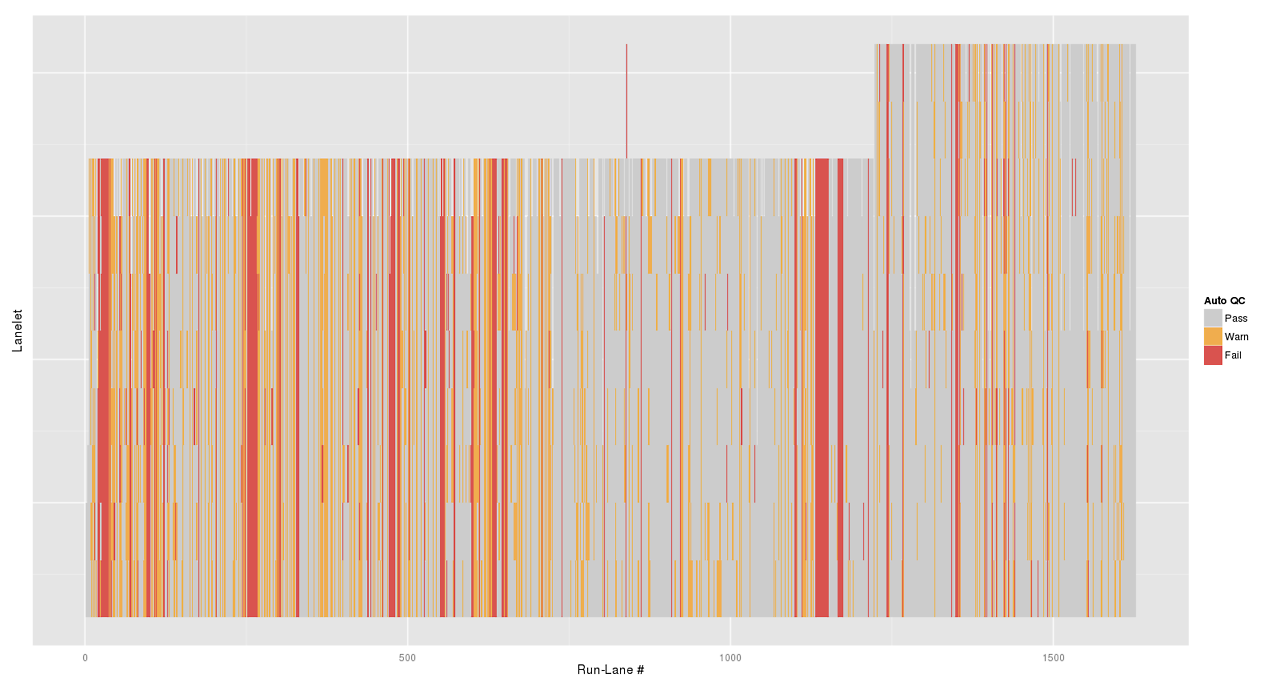
\includegraphics{img/runlane.png}}
\end{frame}

\begin{frame}[t]
\frametitle{Analysis of Current QC System}
    \uncover<1>{
        \begin{beamerboxesrounded}[shadow=true]{}
            \begin{center}
                Frontier
            \end{center}
        \end{beamerboxesrounded}
        \begin{itemize}
            \item My own Python script to read and process these data files
            \item Input formed by output of the current system's statistical data
            \item \texttt{Frontier}'s "StatPlexer" provides an API to access dataframe
        \end{itemize}
    }

    \vskip 0.5cm

    \uncover<2>{
        \begin{beamerboxesrounded}[shadow=true]{}
            \begin{center}
                Rule Extraction
            \end{center}
        \end{beamerboxesrounded}
        \begin{itemize}
            \item Utilising scikit-learn, a Python machine learning framework
            \item Training decision trees on key-value summary statistics
            \item Experimented with various parameter and data handling options
            \item Decision trees prone to overfitting but provide rules to follow
        \end{itemize}
    }
\end{frame}

\begin{frame}[t]
\frametitle{Early Decision Tree}
    \vskip 2.5cm
    \resizebox{1.0\textwidth}{!}{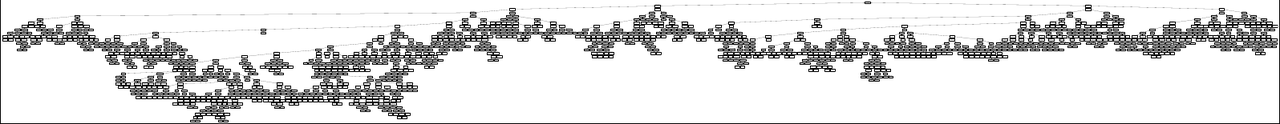
\includegraphics{img/earlytree.png}}
\end{frame}

\begin{frame}[t]
\frametitle{Improved Decision Trees}
    \resizebox{1.0\textwidth}{!}{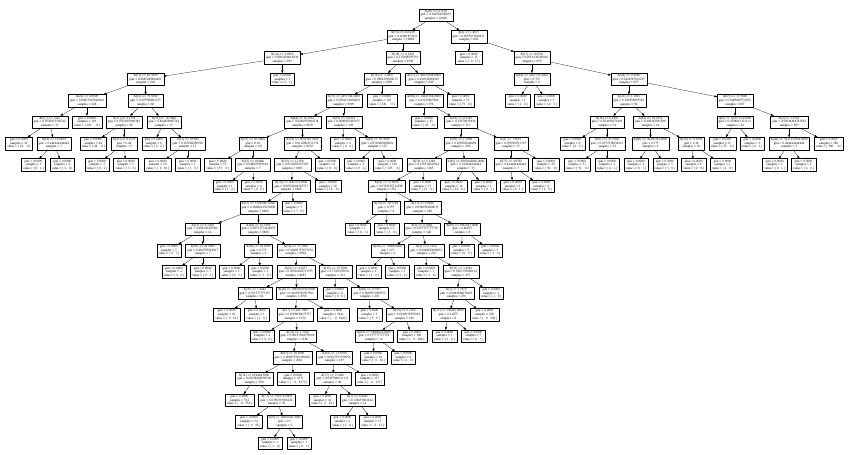
\includegraphics{img/newertree.png}}
\end{frame}

\begin{frame}[t]
\frametitle{Contributions to Current QC System}
\begin{itemize}
    \item \texttt{bamcheckr}; an in-house tool written in R
    \item Supplements \texttt{samtools stats} key-value summary numbers which 
        are then used by the current \texttt{auto\_qc} system

    \vskip 0.5cm

    \begin{beamerboxesrounded}[shadow=true]{}
        \begin{center}
            What did I do?
        \end{center}
    \end{beamerboxesrounded}
    \item Patched a bug that prevented plotting of diagnostic graphs
    \item Writing additional routines to calculate percentage or ratio based 
        parameters that should prove useful for training the decision tree
\end{itemize}
\end{frame}

%%%%%%%%%%%%%%%%%%%%%%%%%%%%%%%%%%%%%%%%%%%%%%%%%%%%%%%%%%% Downstream Progress
\section{Downstream Progress}
\subsection{Downstream Progress}

\begin{frame}[t]
\frametitle{Downstream Progress}
    \begin{beamerboxesrounded}[shadow=true]{}
        \begin{center}
            Variant Call Format (\textbf{VCF})
        \end{center}
    \end{beamerboxesrounded}
    \begin{itemize}
        \item Stores called variant alleles at each location on the genome for 
            each sample; a huge tab delimited file
        \item File also stores reference alleles at these locations and other
            meta-data including quality score and filters
        \item Downloaded and built a collection of tools; \texttt{vcftools} to
            generate indexes and query VCF files for particular columns
    \end{itemize}

    \vskip 0.5cm

    \begin{beamerboxesrounded}[shadow=true]{}
        \begin{center}
            Latest Progress
        \end{center}
    \end{beamerboxesrounded}
    \begin{itemize}
        \item Locations of called variants across all "SNP chips" extracted
        \item Crude Python script to generate candidate regions
    \end{itemize}
\end{frame}


%%%%%%%%%%%%%%%%%%%%%%%%%%%%%%%%%%%%%%%%%%%%%%%%%%%%%%%%%%%%%%%%%%%%%%%% Issues
\section{Issues}
\subsection{Issues}

\begin{frame}[t]
\frametitle{Project Issues: QC Report}
    Some issues encountered so far include:
    \begin{description}
        \item[Data Noise] The "warn" classification seems to introduce a lot of
            noise to the generated decision trees
        \item[CV] Confusion with performing cross-validation with scikit-learn,
            how best to stratify data we have?
        \item[Params] The \texttt{bamcheckr} outputs are missing some percentage
            and ratio formatted parameters that auto\_qc gains from another source
        \item[Pruning] The scikit-learn framework does not support pruning
            of decision trees but analysis of the current trees indicate this
            would provide improvement for generalisation
    \end{description}
\end{frame}

\begin{frame}[t]
\frametitle{Project Issues: Downstream Analysis}
    \begin{description}
        \item[Comms.] A misunderstanding wasted some time as I tried to recover
            strand data for some of the SNP chip data, whilst unnecessary it was
            interesting!
        \item[Region] We need to locate a region of the genome that does not have
            too many or too few variants ("representative")
        \item[CPU] Analysis will require use of Sanger computing clusters due to
            the intensive nature of the variant calling pipeline
        \item[Storage] The size of the candidate region must be not so small as
            to hinder analysis but not too large to avoid computational time and
            storage limitations
    \end{description}
\end{frame}


%%%%%%%%%%%%%%%%%%%%%%%%%%%%%%%%%%%%%%%%%%%%%%%%%%%%%%%%%%%%%%%%%%%%%%%% Future
\section{Future}
\subsection{Future}

\begin{frame}[t]
    \begin{beamerboxesrounded}[shadow=true]{}
        \begin{center}
            What's next?
        \end{center}
    \end{beamerboxesrounded}
    \begin{itemize}
        \item Complete my code for selection of candidate genome regions
        \item Assist construction of Sanger pipeline to perform leave-one-out analysis,
            using candidate region as the target for variant calling
        \item Compare results of this pipeline to the known variants in the
            SNP chips; attempt to determine if there are any effects on accuracy
        \item Can we learn what QC parameters to look for in such cases?
    \end{itemize}

    \vskip 0.5cm

    \begin{beamerboxesrounded}[shadow=true]{}
        \begin{center}
            What else?
        \end{center}
    \end{beamerboxesrounded}
    \begin{itemize}
        \item Refine attempts to replicate current QC rules
        \item Implement new weighting algorithm for cross-validation
        \item Implement pruning for the decision tree
        \item Complete contributions to \texttt{bamcheckr}
    \end{itemize}
\end{frame}

\begin{frame}[t]
    \begin{beamerboxesrounded}[shadow=true]{}
        \begin{center}
            Future
        \end{center}
    \end{beamerboxesrounded}
    \begin{itemize}
        \item Opportunity to patch pruning algorithm in to scikit-learn
        \item Sanger Institute expressed desire to publish research
    \end{itemize}

    \vskip 0.5cm

    \begin{beamerboxesrounded}[shadow=true]{}
        \begin{center}
            With more time...
        \end{center}
    \end{beamerboxesrounded}
    \begin{itemize}
        \item Investigate other machine learning algorithms and their application
            to the learning of quality control classification
        \item Increase the size or even use multiple extracted genomic regions 
            to measure generalisation of what is learned through the leave-one-out
            methodology
    \end{itemize}
\end{frame}

\end{document}

